\documentclass[svgnames,smaller,aspectratio=169]{beamer}

\usepackage{my-theme}
\usepackage{tikz}

\usepackage[normalem]{ulem}
\usepackage{chronology}
\usepackage{fancybox}

\usepackage{amsmath}

\usepackage{biblatex}
%\addbibresource{tutorial.bib}
\bibliography{quantum.bib}

\usepackage{listings}
\lstset{                         %
  language=C++,                  % choose the language of the code
  basicstyle=\ttfamily\small,     % the size of the fonts that are used for the
                                 % code
  numbers=left,                  % where to put the line-numbers
  numberstyle=\footnotesize,     % the size of the fonts that are used for the
                                 % line-numbers.
  stepnumber=1,                  % the step between two line-numbers.
  numbersep=5pt,                 % how far the line-numbers are from the code
  backgroundcolor=\color{gray!6}, % choose the background color. You must add
                                 % \usepackage{color}.
  showspaces=false,              % show spaces adding particular underscores
  showstringspaces=false,        % underline spaces within strings
  showtabs=false,                % show tabs within strings adding particular
                                 % underscores.
  frame=single,                  % adds a frame around the code
  tabsize=2,                     % sets default tabsize to 2 spaces
  breaklines=true,               % sets automatic line breaking
  breakatwhitespace=false,       % sets if automatic breaks should only happen
                                 % at whitespace.
  morekeywords={requires,in,constexpr,string, static_assert},
  keywordstyle=\color{blue}\bfseries,
  commentstyle=\color{Gray},
  stringstyle=\color{red},
  escapeinside={\%*}{*)},         % if you want to add a comment within your code
  captionpos=top,
}
\renewcommand{\lstlistingname}{Code}

\newcommand*{\cpp}{\texttt{C++}}
\newcommand*{\csharp}{\texttt{C\#}}
\newcommand*{\jit}{\texttt{JIT}}

\newcommand{\msmall}{\fontsize{8}{10}\selectfont}

\newcommand*{\ket}{\texttt{C++}}

%% SLIDE INFORMATION------------------------------------------------------------

\title{Introduction to Quantum Computing}
\author{Ugo Jardonnet}
\date{\today}


%-------------------------------------------------------------------------------
\begin{document}
%-------------------------------------------------------------------------------

\begin{frame}
  \titlepage
  %New features of \cpp and how they position in front of managed languages,
  %more precisely \csharp and Java
\end{frame}

\begin{frame}{Table of Contents}
  \tableofcontents
  % You might wish to add the option [pausesections]
\end{frame}

%-------------------------------------------------
\section{A Simple Experiment}
%-------------------------------------------------


\newcommand{\iu}{\mathrm{i}\mkern1mu}

\begin{frame}[fragile]{A Simple Experiment \cite{interfer}}
   \begin{center}
      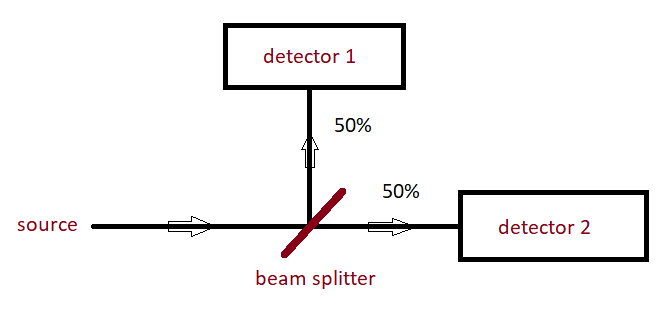
\includegraphics[height=.4\textheight]{exp1}
  \end{center}
  Suppose we have an experimental set-up consisting of a photon source, a beam splitter (half silvered mirror) and a
  pair of photon detectors.  We observe that photons hit each detector 50\% of the time. \\~\
  
  \noindent
  \textbf{The simplest explanation here is that the beam splitter has a 50\% chance to transmit or reflect each photon.}
\end{frame}

\begin{frame}[fragile]{A Simple Experiment \cite{interfer}}
  \begin{center}
      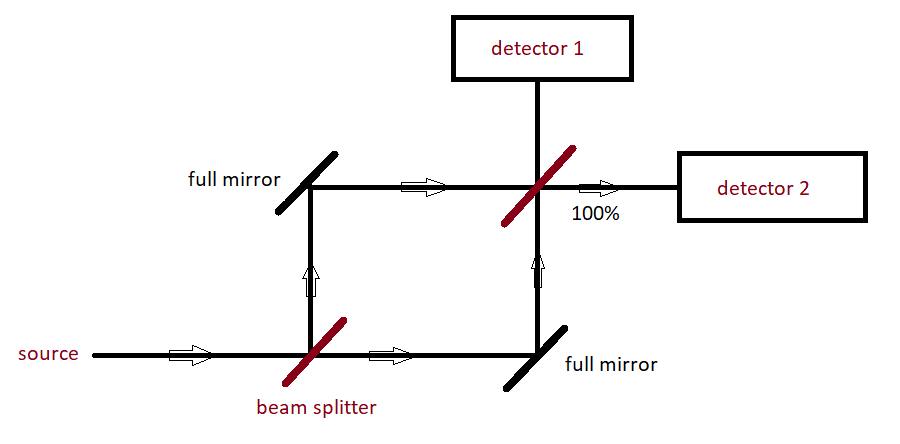
\includegraphics[height=.4\textheight]{exp2}
  \end{center}
  We modify the experiment by adding a second beam splitter and two fully reflecting mirrors.
  In this modified set-up the result is non-intuitive. The photons do not hit each detector with a 50\% chance. \\~\

  \textbf{The photons arrive at the same detector, detector 2, 100\% of the time.}

\end{frame}

\begin{frame}[fragile]{A Simple Experiment \cite{interfer}}
  \textbf{The mathematical framework of quantum physics models the experiment in a way that correctly predicts the
    observed outcomes.}

  The beam splitter can be model by the following operator:
  $\frac{1}{\sqrt{2}}\begin{bmatrix} 1 & \iu \\ \iu & 1 \end{bmatrix}$
  
  At each step, photons can be in 2 possible paths noted $\begin{pmatrix} 1 \\ 0 \end{pmatrix}$ and $\begin{pmatrix} 0 \\ 1 \end{pmatrix}$.

  \begin{enumerate}
  \item At the beginning of the experiment we know from which side photons are hitting the first beam splitter.
    Meaning the state of the system is known to be path 1 $= \begin{pmatrix} 1 \\ 0 \end{pmatrix}$.

  \item After the first beam splitter we get:
    $\frac{1}{\sqrt{2}}\begin{bmatrix} 1 & \iu \\ \iu & 1 \end{bmatrix} \begin{pmatrix} 1 \\ 0 \end{pmatrix} =
    \frac{1}{\sqrt{2}} \begin{pmatrix} 1 \\ \iu \end{pmatrix} =
    \frac{1}{\sqrt{2}} \begin{pmatrix} 1 \\ 0 \end{pmatrix} + \frac{\iu}{\sqrt{2}}\begin{pmatrix} 0 \\ 1 \end{pmatrix}$. \\
    We will see later that this mean a $\bigl(\frac{1}{\sqrt{2}}\bigr)^2= \bigl(\frac{\iu}{\sqrt{2}}\bigr)^2=\frac{1}{2}$ probability for each outgoing path.

  \item After the second beam splitter we get: $\frac{1}{\sqrt{2}}\begin{bmatrix} 1 & \iu \\ \iu & 1 \end{bmatrix}
    \frac{1}{\sqrt{2}} \begin{pmatrix} 1 \\ \iu \end{pmatrix} = \begin{pmatrix} 0 \\ 1 \end{pmatrix}$, meaning a 100\%
    probability of observing photons in path 2.
  \end{enumerate}
\end{frame}

\begin{frame}[fragile]{A Simple Experiment \cite{interfer}}
  \begin{itemize}
  \item FIXME Photons are modeled as taking a superposition of both paths and physical "gates"  as operators modifying the
    probabilities of measuring photons in each of their possible states.
  \end{itemize}
    \begin{itemize}
  \item Quantum physics can model experiment that cannot be described by classical physics.
  \item The exponential processing power needed to model some complex quantum system led to the idea of quantum
    computing.
  \end{itemize}
\end{frame}
  
%-------------------------------------------------
\section{Mathematical Framework}
%-------------------------------------------------

\subsection{Hilbert space and Dirac notation}

\begin{frame}[fragile]{Hilbert space and Dirac Notation}
  The state of a n-qbit system is described by a $2^n$-dimensional vector in a finite dimensional complex vector space,
  referred as a Hilbert space $\mathcal{H}$. \\~\

  Vectors from $\mathcal{H}$ basis are called state vectors. They represent the possible states in which qbits can
  collapse when measured. \\~\
  
  \begin{block}{Dirac Notation}
  %Dirac Notation:
  \begin{itemize}
  \item Vectors in $\mathcal{H}$ are written inside a 'ket' as follow $|v\rangle$
  \item The $2^n$ basis vectors of $\mathcal{H}$ are labeled by their binary index: $ |00\rangle, |01\rangle$, ...
  \end{itemize}
  \end{block}

\end{frame}

\begin{frame}[fragile]{Dirac Notation}

  \begin{block}{Single-qbit System Example}
    Each possible state of a single-qbit system can be written as a vector $\vec{v} = \begin{pmatrix} \alpha_1 \\ \alpha_2 \end{pmatrix}$, with $\alpha_1, \alpha_2$ complex.
    
    Following Dirac notation we get: $ |v\rangle = \alpha_1 |0\rangle + \alpha_2 |1\rangle $
  \end{block}
  
  FIXME boch sphere
\end{frame}

\begin{frame}[fragile]{Dirac Notation}
  
  \begin{block}{4-qbit System Example - $\mathcal{H}$ of dimension 4}
    \begin{center}
      \begin{align*}
        \biggl|\begin{smallmatrix} 0 \\ 1 \\ 0 \\ 0 \end{smallmatrix} & \equiv 2^{nd} \text{ basis vector} \\%[-0.8em]
        & \equiv 0\text{b}01^{th} \text{ basis vector, binary 0-indexed} \\[0.8em]
        & \equiv |01\rangle \text{ in Dirac notation}
      \end{align*}
    \end{center}
    the 4 basis vectors are therefore $\textit{B} = \{|00\rangle, |01\rangle, |10\rangle, |11\rangle\}$. Any vectors in
    $\mathcal{H}$ can then be written as a combination of vectors in $\textit{B}$.
  \end{block}
\end{frame}

\begin{frame}[fragile]{Dirac Notation}
  The following Dirac notation and column vector are equivalent:
  $$\sqrt\frac{2}{3}|001\rangle + \frac{i}{\sqrt(3)}|111\rangle \Longleftrightarrow \begin{pmatrix}0 \\ \sqrt\frac{2}{3}
    \\ 0 \\ \vdots \\ 0 \\ \frac{i}{\sqrt(3)} \end{pmatrix}$$
  As you can see, this notation saves space when the dimension is high and the vectors are sparse.
\end{frame}

\subsection{Operators in $\mathcal{H}$}

\begin{frame}[fragile]{Dual vector and inner product}
    \begin{block}{Dual vector}
       $\langle x |$ - $x$ written inside a 'brac'
    \end{block}
  A dual vector is obtained by taking the corresponding row matrix of $x$ and then the complex conjugate of every
  element (Hermitean conjugate). \\~\

  This allows writing the \textbf{inner product} as $\langle x | y \rangle$:
  \begin{equation*}
    \langle x || y \rangle \equiv \langle x | y \rangle = \begin{pmatrix} x_1 \\ x_2 \end{pmatrix}
    \cdot \begin{pmatrix} y_1 \\ y_2 \end{pmatrix} = (x_1^* x_2^*)\begin{pmatrix} y_1 \\ y_2 \end{pmatrix} =
    \Sigma_i^2x_i^* y_i
    %\text{, where } c^*=a-bi  \text{ for } c=a+bi
  \end{equation*}
   where $c^*=a-bi$  for $c=a+bi$
\end{frame}



\begin{frame}[fragile]{Tensor product}
  \begin{block}{Tensor product}
   $|x\rangle\otimes|y\rangle$ also written $|x\rangle|y\rangle$ or $|xy\rangle$
  \end{block}
  Stitch result matrices of multiplying each element $x_i$ in $x$ by $y$:
$$|xy\rangle = |x\rangle\otimes|y\rangle = \begin{pmatrix} x_0 \\ x_1 \end{pmatrix} \otimes \begin{pmatrix} y_0 \\ y_1 \end{pmatrix}
  = \begin{pmatrix} x_0 y_0 \\ x_0 y_1 \\ x_1 y_0 \\ x_1 y_1 \end{pmatrix}$$
  
Example: $$\sqrt\frac{2}{3}|01\rangle + \frac{i}{\sqrt(3)}|11\rangle \Longleftrightarrow \sqrt\frac{2}{3}|0\rangle\otimes|1\rangle + \frac{i}{\sqrt(3)}|1\rangle\otimes|1\rangle$$
\end{frame}

\begin{frame}[fragile]{Outer product}
  dsfs
\end{frame}


%-------------------------------------------------
\section{Quantum Algorithm}
%-------------------------------------------------

\subsection{Shor's algorithm}

\begin{frame}[fragile]{Shor's Algorithm}
  test
\end{frame}


\subsection{Groover's algorithm}
\begin{frame}[fragile]{Groover's Algorithm}
test
\end{frame}

\section*{Bibliography}
\begin{frame}[allowframebreaks]{Bibliography}
\printbibliography
\end{frame}

\end{document}
